\documentclass[
  % all of the below options are optional and can be left out
  % course name (default: 2IL50 Data Structures)
  course = {{IE579 Game Theory and Multi-Agent Reinforcement Learning}},
  % quartile (default: 3)
  quartile = {{4}},
  % assignment number/name (default: 1)
  assignment = 2,
  % student name (default: Some One)
  name = {{Mohammad Mahdi Rahimi}},
  % student number, NOT S-number (default: 0123456)
  studentnumber = {{20208244}},
  % student email (default: s.one@student.tue.nl)
  email = {{mahi@kaist.ac.kr}},
  % first exercise number (default: 1)
  firstexercise = 1
]{aga-homework}

\usepackage{amssymb,latexsym,amsmath,amsthm}
\usepackage{amsfonts,rawfonts}
\usepackage{thmtools}
\usepackage{systeme}
\usepackage{mathtools}
\usepackage{xcolor}
\usepackage{pgfplots} 
\usepackage{amsmath}
\usepackage{algorithm}
\usepackage{cancel}
\usepackage[noend]{algpseudocode}
\usepackage{minted}
\usepackage{tikz}
\usetikzlibrary{calc}
\usepackage[dvipsnames]{xcolor}
% \usepackage[margin=1.5in]{geometry}    % For margin alignment


\pgfplotsset{width=10cm,compat=1.9} 
 \usepgfplotslibrary{external}

\tikzexternalize 
% \tikzset{
%   % Two node styles for game trees: solid and hollow
%   solid node/.style={circle,draw,inner sep=2,fill=black},
%   hollow node/.style={circle,draw,inner sep=2},
%   empty node/.style={rectangle,draw,fill=white,color=white}
% }

% macro for entering payoffs
\newcommand\payoff[1]{
  $\begin{pmatrix} #1 \end{pmatrix}$
}



\begin{document}

\exercise
\subexercise $x = 1$ Find Pure Nash and SPE
\\\\
Nash Equilibrium :\\
1. \{(R,G),(U)\}\\
2. \{(R,H),(U)\}\\
3. \{(L,G),(D)\}\\
4. \{(L,H),(D)\}\\
\\
Sub-game Perfect Nash Equilibrium :\\
1. \{(R,H),(U)\}


\subexercise Range of x for having (R, U) as unique SPE
\\\\
For $x > 2$ player-1 choose $(L)$, and for $x = 2$ player-1 is indifferent between $(L)$ and $(R)$ in sub-game, so for the range of $x < 2$, $(R, U)$ is the unique SPE.
\\\\
\subexercise  Range of x for having (L) as unique SPE
\\\\
For $x > 2$ player-1 choose $(L)$, and it is the unique SPE.

\exercise
\subexercise All Pure Nash
\\\\
Player-1 Actions: $\{L, C, R\}$\\
Player-2 Actions: $\{U, D\}$\\
Converting game to a normal-form(3x2) we find following pure Nash equilibrium:\\
1. $(R, U) = (5, 5)$\\
2. $(C, D) = (5, 5)$

\subexercise Mixed Nash Equilibrium \\\\
For finding mixed equilibrium we randomize over pure solutions actions:\\
Player-1 Plays: $P\{R\} + (1 - P)\{C\}$\\
Player-2 Plays: $Q\{U\} + (1 - Q)\{D\}$\\
So we get:\\
\begin{equation} \label{eq1}
\begin{split}
& PQ\{R, U\} + (1 - P)Q\{C, U\} + p(1 - Q)\{R, D\} + (1 - P)(1 - Q)\{C, D\} \\
= & PQ\{5, 5\} + (1 - P)Q\{0, 0\} + P(1 - Q)\{-15, -15\} + (1 - P)(1 - Q)\{5, 5\}\\
\Rightarrow &   \begin{cases}
      U_1 = 5PQ + -15P(1 - Q) + 5(1 - P)(1 - Q) = 25PQ - 20P - 5Q + 5 = P(25Q - 20) - 5Q + 5 \\
      U_2 = 5PQ + -15P(1 - Q) + 5(1 - P)(1 - Q) = 25PQ - 20P - 5Q + 5 = Q(25Q - 5) - 20P + 5 \\
     \end{cases}
\end{split}
\end{equation}\\
By looking at best response for each Player:
\begin{equation} \label{eq1}
\begin{split}
BR_1 & = \begin{cases}
      P = 1 if  Q > \frac{20}{25} \\
      P = 0 otherwise\\
     \end{cases}\\
BR_2 & = \begin{cases}
      Q = 1\text{ if  }P > \frac{5}{25} \\
      Q = 0\text{ Otherwise }\\
     \end{cases}\\
\end{split}
\end{equation}\\
Therefore Two Intersect of Best-Response are (P = 1, Q = 1) and (P = 0, Q = 0) which are same as pure Nash solutions.

\subexercise Behavioral Strategy
Player-1 Actions: $\{L, C, R\}$\\
Player-2 Actions: $\{U, D\}$\\

For finding behavioral equilibrium we randomize over all actions:\\
Player-1 Plays: $P_L\{L\} + P_C\{C\} + P_R\{R\} \text{ ,  } \sum{P} = 1$\\
Player-2 Plays: $Q_U\{U\} + Q_D\{D\} \text{ ,  } \sum{Q} = 1$\\

By considering equilibrium of (C-R) forest, it is either RU or CD, we do not need to randomize over Q and over (R,C), we can randomize over RU and CD which has same outcome.

One the other hand, LC is always dominated by LL and LR, so we can assume that we don't need to give C any chance and player-1 can always randomize between L and R to receive maximum outcome of behavioral.

C is not a best-response, so we exclude it.

Player-1 Plays: $P\{L\} + (1 -P)\{R\}$\\

So we have utility functions as below:
\begin{equation} \label{eq1}
\begin{split}
& U_1 = U_2 = P^2 + 10P(1-P) + 5(1-P) = -9P^2 + 5P + 5 \\
\textbf{Maximizing} \Rightarrow & -18P + 5 = 0 \Rightarrow P = \frac{5}{18}\\
\Rightarrow & max(U_2) = max(U_1) = 5.695
\end{split}
\end{equation}\\
highest expected happen when Player-1 randomize by $\{\frac{5}{18}L, \frac{13}{18}R\}$ and Player-2 always $\{U\}$.


\exercise
\subexercise 
\\\\
If mentioned strategy $(S)$ wants to be a sub-game perfect equilibrium, it has to have a better payoff than any other derivation of strategy $(S^\prime)$. 
\begin{equation} \label{eq1}
\begin{split}
U_i(S^\prime) \le U_i(S) \\
\end{split}
\end{equation}\\
And we have utilities as follows:\\
\begin{equation} \label{eq1}
\begin{split}
U_1(S) & = (1 - \delta)\sum^\infty_{t = 1}{4\delta^{t - 1}} = 4 - \frac{4\delta}{1 - \delta} = (1 - \delta)\frac{4}{1 - \delta} = 4\\
U_1(S^\prime) & = (1 - \delta)(6 + \sum^\infty_{t = 1}{\delta^{t - 1}} - 1) = 5(1 - \delta) + 1 = 6 - 5\delta\\
\end{split}
\end{equation}\\
By replacing (5) in (4) we get:
\begin{equation} \label{eq1}
\begin{split}
6 - 5\delta \le & 4\\
-5\delta \le & -2\\
\frac{2}{5} \le & \delta
\end{split}
\end{equation}\\

\subexercise
\\\\
If mentioned Tit-for-Tat strategy $S$ wants to be a sub-game perfect equilibrium, it has to have a better payoff than any other derivation of strategy $(S^\prime)$.
\begin{equation} \label{eq1}
\begin{split}
U_1(S) & = (1 - \delta)\sum^\infty_{t = 1}{4\delta^{t - 1}} = 4\\
U_1(S^\prime) & = (1 - \delta)(6 + \sum^{\infty}_{t = 1}{6\delta^{2t}} + \sum^\infty_{t=1}{0 \delta^{2t-1}}) = 6(1 - \delta)(1 + \sum^{\infty}_{t = 1}{\delta^{2t}}) \\
& = 6(1 - \delta)(\sum^{\infty}_{t = 0}{\delta^{2t}})
\end{split}
\end{equation}\\
First, we proof that $(\sum^{\infty}_{t = 0}{\delta^{2t}})$ is equal $\frac{1}{1 - \delta^2}$ for $0 < \delta < 1$:
\begin{equation} \label{eq1}
\begin{split}
\sum^{\infty}_{t = 0}{\delta^{t}} & = \sum^{\infty}_{t = 0}{\delta^{2t}} + \sum^{\infty}_{t = 0}{\delta^{2t+1}} = \frac{1}{1 - \delta}\\
\end{split}
\end{equation}\\
\begin{equation} \label{eq1}
\begin{split}
\sum^{\infty}_{t = 0}{\delta^{2t}} - \sum^{\infty}_{t = 0}{\delta^{2t+1}} = \sum^{\infty}_{t = 0}{\delta^{2t} - \delta^{2t+1}} = (1 - \delta)\sum^{\infty}_{t = 0}{\delta^{2t}}\\
\end{split}
\end{equation}\\
By using (8) and (9):\\
\begin{equation} \label{eq1}
\begin{split}
& 2\sum^{\infty}_{t = 0}{\delta^{2t}} = \frac{1}{1 - \delta} + (1 - \delta)\sum^{\infty}_{t = 0}{\delta^{2t}}\\
\Rightarrow & (1 + \delta)\sum^{\infty}_{t = 0}{\delta^{2t}} = \frac{1}{1 - \delta}\\
\Rightarrow & \sum^{\infty}_{t = 0}{\delta^{2t}} = \frac{1}{1 - \delta^2}\\
\end{split}
\end{equation}\\
By applying (10) in (7):\\
\begin{equation} \label{eq1}
\begin{split}
U_1(S) & = 4\\
U_1(S^\prime) & = 6(1 - \delta)(\frac{1}{1 - \delta^2}) = \frac{6}{1 + \delta}
\end{split}
\end{equation}\\
By replacing (11) in (4) we get:
\begin{equation} \label{eq1}
\begin{split}
\frac{6}{1 + \delta} \le & 4\\
6 \le & 4 + 4\delta\\
2 \le & 4\delta\\
\frac{1}{2} \le \delta
\end{split}
\end{equation}\\

\exercise
\subexercise Extensive Form of game
\\\\
\begin{center}
\begin{tikzpicture}[scale=1.5]
\tikzset{
h/.style={circle,draw=magenta,thick,inner sep=1.5},
s/.style={h,fill=magenta}
}
\tikzstyle{level 1}=[level distance=15mm, sibling distance=50mm]
\tikzstyle{level 2}=[level distance=15mm, sibling distance=20mm]
\tikzstyle{level 3}=[level distance=15mm, sibling distance=7mm]
\node(0)[s, label=above:Nature]{}
    child{node(1a)[s, label=above:1]{}
        child{node(2aa)[s, label=left:2]{}
            child{node(3aaa)[h, label=below:0]{} edge from parent node[left]{$R$}}
            child{node(3aab)[h, label=below:-1]{} edge from parent node[left]{$P$}}
            child{node(3aac)[h, label=below:1]{} edge from parent node[left]{$S$}}
            edge from parent node[left]{$R$}
        }
        child{node(2ab)[s, label=left:2]{}
            child{node(3aba)[h, label=below:1]{} edge from parent node[left]{$R$}}
            child{node(3abb)[h, label=below:0]{} edge from parent node[left]{$P$}}
            child{node(3abc)[h, label=below:-1]{} edge from parent node[left]{$S$}}
            edge from parent node[left]{$P$}
        }
        child{node(2ac)[s, label=left:2]{}
            child{node(3aca)[h, label=below:-1]{} edge from parent node[left]{$R$}}
            child{node(3acb)[h, label=below:1]{} edge from parent node[left]{$P$}}
            child{node(3acc)[h, label=below:0]{} edge from parent node[left]{$S$}}
            edge from parent node[left]{$S$}
        }
        edge from parent node[left]{$a$}
    }
    child{node(1b)[s, label=above:1]{}
        child{node(2ba)[s, label=left:2]{}
            child{node(3baa)[h, label=below:-1]{} edge from parent node[left]{$R$}}
            edge from parent node[left]{$P$}
        }
        child{node(2bb)[s, label=left:2]{}
            child{node(3bba)[h, label=below:0]{} edge from parent node[left]{$P$}}
            edge from parent node[left]{$P$}
        }
        child{node(2bc)[s, label=left:2]{}
            child{node(3bca)[h, label=below:1]{} edge from parent node[left]{$S$}}
            edge from parent node[left]{$P$}
        }
        edge from parent node[left]{$1 - a$}
    };

\draw[dashed, rounded corners=10]($(1a) + (-0.2, 0.25)$)rectangle($(1b) + (0.2, -0.25)$)
\end{tikzpicture}
\end{center}

\subexercise Normal-Form representation
\\\\
\begin{center}
\begin{tabular}{ |c|c|c|c| } 
\hline 
 & R & P & S \\
\hline
(P,R) & $a - 1$ & $a$ & $1 - 2a$ \\ 
\hline
(P,P) & -1 & 0 & 1 \\ 
\hline
(P,S) & $2a - 1$ & $-a$ & $1 - a$ \\ 
\hline
\end{tabular}   if $a = \frac{1}{3} \Rightarrow$
\begin{tabular}{ |c|c|c|c| } 
\hline 
 & R & P & S \\
\hline
(P,R) & $-\frac{2}{3}$ & $\frac{1}{3}$ & $\frac{1}{3}$ \\ 
\hline
(P,P) & -1 & 0 & 1 \\ 
\hline
(P,S) & $-\frac{1}{3}$ & $-\frac{1}{3}$ & $\frac{2}{3}$ \\ 
\hline
\end{tabular}    
\end{center}

\subexercise Find Nash Equilibrium
\\\\
Playing $S$ is dominant strategy for player 1, and player-2 best responce is $(P,R)$ to we have a Bayesian Nash on: $\{S, (P,R)\}$ with payoff of $\frac{1}{3}$.

\exercise
\subexercise
\\\\
If row agent randomize action by $P$ over $\{U, D\}$ and columns agent by $Q$ over $\{L, R\}$, then the Payoff for agents is as follows:
\begin{equation} \label{eq1}
\begin{split}
U_1 & = P(1 - Q) + 2(1 - P)Q = P + 2Q - 3PQ \\
U_2 & = 6PQ + 2P(1 - Q) + (1 - P)Q = 2P + Q + 3PQ
\end{split}
\end{equation}\\
Find the minmax points by derivations:
\begin{equation} \label{eq1}
\begin{split}
maximin(U_1) = \begin{cases}
      \frac{\partial U_1}{\partial P} \rightarrow 1 - 3Q \rightarrow Q = \frac{1}{3}\textbf{ minimize the utility }\\
      \frac{\partial U_1}{\partial Q} \rightarrow 2 - 3P \rightarrow P = \frac{2}{3}\textbf{ maximize the utility }\\
     \end{cases}\\
maximin(U_2) = \begin{cases}
      \frac{\partial U_2}{\partial P} \rightarrow 2 + 3Q \rightarrow Q = 1\textbf{ maximize the utility }\\
      \frac{\partial U_2}{\partial Q} \rightarrow 1 + 3P \rightarrow P = 0\textbf{ minimize the utility }\\
     \end{cases}\\
\end{split}
\end{equation}\\
Maximin strategy for Player-2 is $\frac{2}{3}U + \frac{1}{3}D$ with payoff of $\frac{2}{3}$ and other can enforce it by playing $\frac{1}{3}L + \frac{2}{3}R$.
\\
Maximin strategy for Player-2 is $L$ with payoff of $1$ and other can enforce it by playing $D$.


\subexercise Achievable and Enforceable Area\\
Achievable area is a convex area of pure strategy outcomes.
\begin{center}
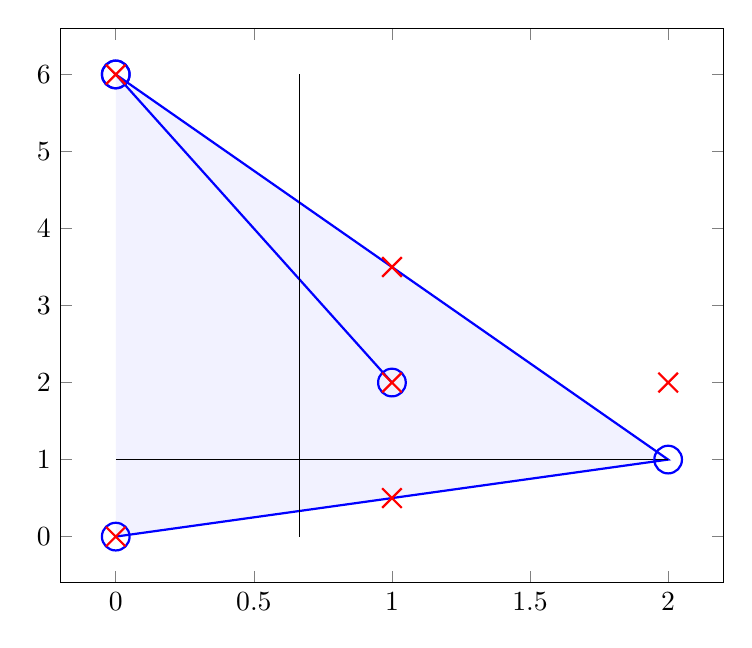
\begin{tikzpicture} 
    \begin{axis}[enlargelimits=0.1]
        \addplot [thick,color=blue,mark=o,fill=blue, 
                    fill opacity=0.05,mark size=5pt]coordinates {
            (0, 0) 
            (2, 1)
            (0, 6)
            (1, 2)
            (0,6)};
        \addplot [only marks,thick,color=red,mark=x,mark size=5pt]coordinates {
            (0, 0) 
            (0, 6)
            (1, 2)
            (1, 3.5)
            (1, 0.5)
            (2, 2)};
            \addplot [
    domain=0:2, 
    samples=100, 
    color=black,
    ]
    {1};
    \addplot +[mark=none, black] coordinates {(2/3, 0) (2/3, 6)};
    \end{axis}
\end{tikzpicture}  
\end{center}
(1, 2) and (1, 3.5) are both Achievable and Enforceable.

\subexercise Find Nash for Payoff of (1,3)
\\\\
\begin{equation} \label{eq1}
\begin{split}
(1,3) & \Rightarrow \begin{cases}
       P + 2Q - 3PQ = 1\\
       2P + Q + 3PQ = 3\\
     \end{cases} \Rightarrow 3P + 3Q = 4 \Rightarrow P = \frac{4}{3} - Q \\
& \Rightarrow \frac{4}{3} - Q + 2Q - 3(\frac{4}{3} - Q)Q = 1 \\
& \Rightarrow \frac{1}{3} + 1Q - 4Q + 3Q^2 = 0 \\
\end{split}
\end{equation}
\begin{equation} \label{eq1}
\begin{split}
& \Rightarrow Q^2 - Q + \frac{1}{9} = 0 \Rightarrow \begin{cases}
       Q = 0.87, P = \frac{4}{3} - 0.87 = 0.46 \textbf{ True Answers}\\
       Q = 0.13, P = \frac{4}{3} - 0.13 = 1.20 \textbf{ Out of Bounds}\\
     \end{cases}\\
& \Rightarrow \begin{cases}
       Q = 0.87\\
       P = 0.46\\
     \end{cases}\\
\end{split}
\end{equation}\\
If anyone derivate from this Nash, other player enforce the minimum payoff for that player as punishment.

\exercise
\\\\
Extensive-Form representation
\begin{center}
\begin{tikzpicture}[scale=1.5]
\tikzset{
h/.style={circle,draw=magenta,thick,inner sep=1.5},
s/.style={h,fill=magenta}
}
\tikzstyle{level 1}=[level distance=15mm, sibling distance=40mm]
\tikzstyle{level 2}=[level distance=15mm, sibling distance=20mm]
\tikzstyle{level 3}=[level distance=15mm, sibling distance=10mm]
\node(0)[s, label=above:Nature]{}
    child{node(1a)[s, label=above:1]{}
        child{node(2aa)[s, label=left:2]{}
            child{node(3aaa)[h, label=below:{$(2,1)$}]{} edge from parent node[left]{$B$}}
            child{node(3aab)[h, label=below:{$(0,0)$}]{} edge from parent node[left]{$S$}}
            edge from parent node[left]{$B$}
        }
        child{node(2ab)[s, label=left:2]{}
            child{node(3aba)[h, label=below:{$(0,0)$}]{} edge from parent node[left]{$B$}}
            child{node(3abb)[h, label=below:{$(1,2)$}]{} edge from parent node[left]{$S$}}
            edge from parent node[left]{$S$}
        }
        edge from parent node[left]{$\frac{1}{2}$}
    }
    child{node(1b)[s, label=above:1]{}
        child{node(2ba)[s, label=left:2]{}
            child{node(3baa)[h, label=below:{$(2,0)$}]{} edge from parent node[left]{$B$}}
            child{node(3baa)[h, label=below:{$(0,2)$}]{} edge from parent node[left]{$S$}}
            edge from parent node[left]{$B$}
        }
        child{node(2bb)[s, label=left:2]{}
            child{node(3bba)[h, label=below:{$(0,1)$}]{} edge from parent node[left]{$B$}}
            child{node(3bba)[h, label=below:{$(1,0)$}]{} edge from parent node[left]{$S$}}
            edge from parent node[left]{$S$}
        }
        edge from parent node[left]{$\frac{1}{2}$}
    };

\draw[dashed, rounded corners=10]($(1a) + (-0.2, 0.25)$)rectangle($(1b) + (0.2, -0.25)$)
\end{tikzpicture}
\end{center}

Normal-Form representation
\begin{center}
\begin{tabular}{ |c|c|c|c|c| } 
\hline 
 & BB & BS & SB & SS \\
\hline
B & $(2, 0.5)$ & $(2, 1.5)$ & $(1, 0)$ & $(0, 1)$ \\ 
\hline
S & $(0, 0.5)$ & $(0.5, 0)$ & $(0.5, 1.5)$ & $(1, 1)$ \\ 
\hline
\end{tabular}    
\end{center}

Find Nash Equilibrium
\\\\
We have Bayesian Nash on $\{(B, BS\}$, so no one will derivate from that actions.


\exercise
\subexercise Find Equilibrium
\begin{equation}
    \begin{split}
        \begin{cases}
        U_1 = q_1(a - q_1 - q_2 - C) = (a - C)q_1 - q_2q_1 - q^2_1\\
        U_2 = q_2(a - q_1 - q_2 - C) = (a - C)q_2 - q_1q_2 - q^2_2\\
        \end{cases}\\
    \end{split}
\end{equation}\\
The Best Response for player-2 can be shown as follows:\\
\begin{equation}
    \begin{split}
        & \frac{\partial U_2}{\partial q_2} = (a - C) - q_1 - 2q_2 = 0\\
        \Rightarrow & q^*_2 = \frac{a - c - q_1}{2}
    \end{split}
\end{equation}\\
One the other hand, firm-1 is not certain about cost of firm-2 to utility of firm-1 can be described as below:\\
\begin{equation}
    \begin{split}
        U_1 = (a - C)q_1 - (\theta q^*_L + (1 - \theta) q^*_H)q_1 - q^2_1\\
    \end{split}
\end{equation}\\
So the best response of firm-1 is:
\begin{equation}
    \begin{split}
        & \frac{\partial U_1}{\partial q_1} = a - C - \theta q^*_L - (1 - \theta) q^*_H - 2q_1 = 0\\
        \Rightarrow & q^*_1 =  \frac{1}{2}(a - C - \theta q^*_L - (1 - \theta) q^*_H)
    \end{split}
\end{equation}\\
By replacing (18) in (20) we have:
\begin{equation}
    \begin{split}
        q^*_1 & =  \frac{1}{2}(a - C - \theta \frac{a - C_L - q^*_1}{2} - (1 - \theta) \frac{a - C_H - q^*_1}{2})\\
        2q^*_1 - \frac{1}{2}q^*_1 & = \frac{1}{2}(a - 2C + \theta C_L + (1 - \theta) C_H)\\
        q^*_1 & = \frac{1}{3}(a - 2C + \theta C_L + (1 - \theta) C_H)\\
        \Rightarrow q^*_H & =  \frac{1}{3}(a - 2C_H + C)\\
        \Rightarrow q^*_L & =  \frac{1}{3}(a - 2C_L + C)\\
        \Rightarrow q^*_2 & =  \frac{1}{3}(a - C)
    \end{split}
\end{equation}\\
By replacing (21) in utilities:
\begin{equation}
    \begin{split}
        & \begin{cases}
        U_1 = (a - C)q_1 - q_2q_1 - q^2_1 > 0\\
        U_2 = (a - C)q_2 - q_1q_2 - q^2_2 > 0\\
        \end{cases} \Rightarrow \begin{cases}
        a - C - q_2 - q_1 > 0\\
        a - C - q_1 - q_2 > 0\\
        \end{cases} \Rightarrow a - C > q_1 + q_2\\
    \end{split}
\end{equation}\\
By replacing (21) in (22):
\begin{equation}
    \begin{split}
        a - C & > \frac{1}{3}(a - 2C + \theta C_L + (1 - \theta C_H) + \frac{1}{3}(a - C)\\
        2a - 2C & > a - 2C + \theta C_L + (1 - \theta) C_H\\
        a & > \theta C_L + (1 - \theta) C_H + (2\theta - 1)C_L - (2\theta - 1)C_L\\
        a & > (1 - \theta) C_L + (1 - \theta) C_H + (2\theta - 1)C_L \\
        C_H - C_L & < \frac{a - (2\theta - 1)C_L}{1 - \theta} \textbf{ Upper bound to have positive utility for both firm }
    \end{split}
\end{equation}
\subexercise
\begin{equation}
    \begin{split}
    q^*_1 = & \begin{cases}
        \frac{1}{3}(a - 2C + C_L) \text{ if } C_2 = C_L\\
        \frac{1}{3}(a - 2C + C_H) \text{ if } C_2 = C_H\\
        \end{cases} \\\\
    \Rightarrow & q^L_1 \le q^*_1 \textbf{ and } q^H_1 \ge q^*_1 
    \end{split}
\end{equation}


\exercise


\exercise



\end{document}
